\maketitle

%\cleardoublepage
%\thispagestyle{plain}
%\vspace*{\fill}
%\begin{center}
%	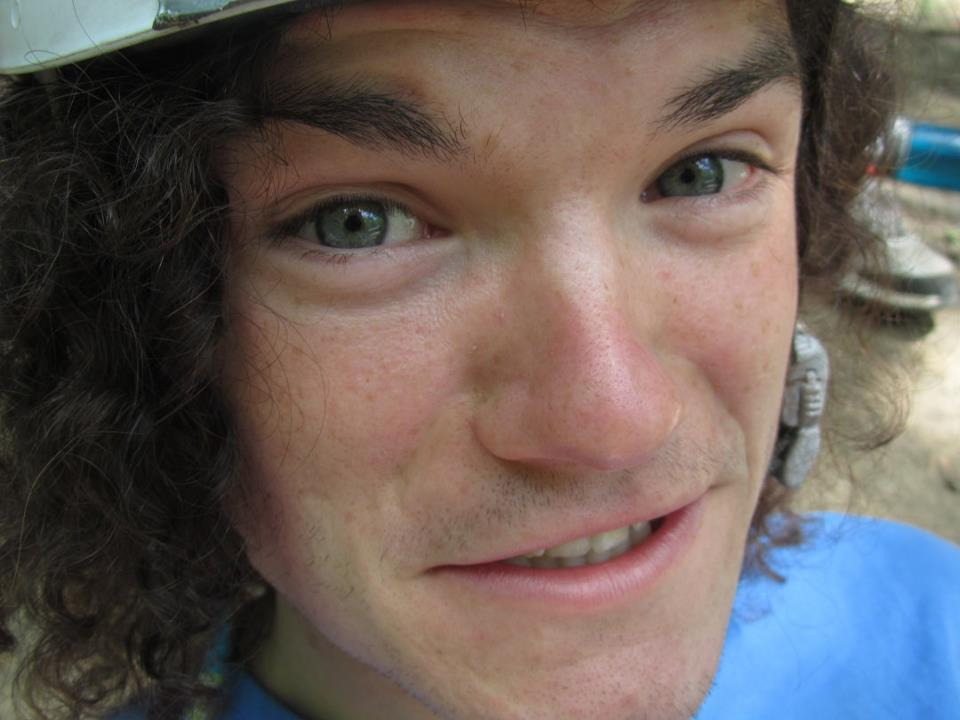
\includegraphics[width=0.8\textwidth]{Images/seanFace.jpg}
%	\newline
%	\newline
%	\Huge
%	Welcome to my thesis, are your ready for some fun?
%	\normalsize
%\end{center}
%\vspace*{\fill}

\begin{abstract}
	Timbre is the property of a sound which allows it to be distinguished from other sounds of the same loudness and
	pitch. These differences can also be demonstrated mathematically using various low level signal features.  Research
	into timbre typically focusses on analysing the multidimensional relationship between these low level features and
	the perceived timbre. In music production, the timbre of recorded sounds is altered through the application of audio
	effects. A commonly used class of audio effects is harmonic excitation, in which new spectral content is introduced
	to the signal at harmonic frequencies. This thesis focusses on the uses of harmonic excitation effects for the
	control of timbre. For a harmonic excitation system to provide control over the timbre of a signal it must be able
	to manipulate the associated low level features. As such, a novel methodology is proposed for evaluating the
	performance of harmonic excitation algorithms, describing how well they are suited to applying timbral control. It
	is found that the most flexibility is provided by methods which allow for the generation of individual harmonics.

	Generating individual harmonics allows for the reconstruction of signals from which harmonic content has been lost
	through degradation. Of the harmonic excitation algorithms evaluated for use in timbral control, three can be used
	to generate individual harmonics. The perceptual quality of these algorithms is assessed through listening tests in
	which participants grade reconstructed signals. It is found that increasing the computational complexity of the
	algorithms (using higher order filters, or longer windows for spectral analysis) improves the quality of the
	reconstruction.
	
	In music production, timbral manipulations are often described using semantic descriptors (e.g. `warm' and
	`bright'). The timbral meanings of these terms can be discerned through analysis of the relationship between their
	use to describe audio signals and the signal's low level features. To investigate these relationships a study is
	conducted analysing the changes to perceived timbre and audio features associated with the application of distortion
	and equalisation effects. This study utilises data collected using a novel methodology in which data is collected as
	part of the music production workflow. Four distinct timbral groups are identified (warmth, brightness, crunchiness
	and muddiness) each consisting of related semantic terms. The perceptual meanings of these semantic groups are
	uncovered by measuring how the low level features of signals are manipulated by the application of the effects. The
	distinction between each of the groups are found to be highly correlated with several low level audio features.
	
	Significant experience is required to be able to utilise traditional studio equipment to manipulate the timbre of a
	sound based on a semantic description. Recently, new tools have been developed which have control parameters
	labelled with commonly used timbral descriptors, reducing the amount of experience needed. These systems manipulate
	the low level features of a signal associated with a particular timbral descriptor. In this work, novel techniques
	are developed by which harmonic excitation algorithms can be used to provide monotonic control over various low
	level features of audio signals. These are then used to build two systems which manipulate timbre based on two
	timbral groups: one moving audio between the warmth and brightness timbral groups and the other between the
	brightness and crunchiness groups. The muddiness group was discarded due to insufficient information. Subjective
	listening tests are conducted to evaluate the performance of these systems. Both are successful in processing audio
	such that it is perceived as part of the brightness group, participants exhibiting a minimum accuracy of 72\% in
	identifying the relevant timbral group. When configured to introduce warmth or crunchiness the systems perform less
	well, participants only identifying the correct timbral group 54\% or 51\% of the time respectively.
\end{abstract}

\begin{acknowledgements}
	Firstly I would like to thank my supervisors Ryan Stables and Cham Athwal for their support and guidance throughout
	my PhD. You are both a continued source of inspiration and have allowed me to work in my own way from the outset.
	Additionally a number of other people within the lab have provided me with much needed academic / emotional support:
	the Orca Pod (Sam Smith, Matthew Cheshire, Muadh Al-Kalbani and Alan Do\l{}hasz), Xueyang Wang, Nick Jillings,
	Spyros Stasis, Ian Williams, Dominic Ward, Greg Hough and Carl Southall. Among you there is always somebody I can
	come to with questions or drag to the pub for a pint. An extra thanks to all the other past and present members of
	the DMT lab, you lot make it a genuine pleasure to come into the office every day. Thanks also to Josh Reiss, Jamie
	Bullock and Zlatko Baracskai who all provided input into my work at various stages.

	Lastly, a massive thanks to my family for generally just being the loveliest bunch of people around.

	\begin{center}
		
\includegraphics[width=0.3\textwidth]{Images/orca.pdf}
	\end{center}
\end{acknowledgements}

\tableofcontents
\listoffigures
\listoftables
\listof{datum}{List of Data}
\printglossaries
\cleardoublepage
